\chapter{Legolas applications} \label{ch: legolas_applications}


\graphicspath{{05-applying_legolas/figures/}}

\begin{chapterquote}[Robert C. Martin][Clean Code: A Handbook of Agile Software Craftsmanship][]
  Why do most developers fear to make continuous changes to their code? Because they are afraid they'll break it.
  Why are they afraid they'll break it? Because they don't have tests.
\end{chapterquote}

\usespublishedwork{
  Most of this Chapter was published in ``Legolas: a novel tool for magnetohydrodynamic spectroscopy'', 2020, \apjs,
  251, 25 \citep{claes2020_legolas}. N. Claes developed {\legolas} in close collaboration with J. De Jonghe, generated the data and figures and wrote a first draft of the manuscript; J. De Jonghe revised and extended the manuscript. R. Keppens contributed to the revision of the paper.
}

In the previous Chapter we discussed the mathematical formalism behind {\legolas}. As is common practice when developing a brand new numerical code we now have to test the implementation against various known results. This Chapter will mostly be dedicated to the validation of our new numerical tool, by comparing numerical spectra with known results from theory and/or the literature. Additionally, we will briefly touch upon the extensive (and continuous) testing framework {\legolas} uses.

\section{Introduction}
Any piece of software, both existing and newly developed, should be accompanied by a decent testing framework to ensure that any changes made to the code, either in the present or in the future, do not break things that were previously working fine. It is easy to develop a piece of code, it is less easy to develop a \emph{working} piece of code, and finally it is certainly not enough for code to just ``work''. Every part of the implementation should be tested against known results in order to make sure that the code actually does what it is expected to do. In an ideal world, every single line of a code base is tested at least once, while at the same time also accounting for various branches in the logic.

In this Chapter we validate {\legolas} against a plethora of test cases, thereby ensuring a correct treatment of the governing equations. Depending on which physical effects are taken into account, we know a priori some general spectral properties that should hold, and we can thus test the properties of the obtained spectra against our predictions. For eigenmode quantifications of ideal, static MHD configurations under adiabatic conditions, we know that the static -- that is, no equilibrium flow -- and adiabatic linear MHD equations make the problem self-adjoint. When performing a standard Fourier analysis in the ignorable directions, the resulting eigenvalue problem is then Hermitian, meaning that all eigenfrequencies will be either fully real (stable waves) or fully complex (pure damped or unstable modes), hence they are found on the real or imaginary axis of the complex eigenfrequency plane, and the full MHD spectrum will be both left-right and up-down symmetric. The inclusion of nonideal effects like resistivity or thermal conduction lifts the self-adjointness of the eigenvalue problem, allowing the eigenmodes to move away from the axes into the complex plane, and the up-down symmetry gets broken. As long as the equilibrium configuration is static, all (adiabatic or non-adiabatic) modes will still have a complementary mode that lies mirrored around the imaginary axis, making the entire spectrum left-right symmetric. This is related to the forward and backward propagating mode symmetry, or the equivalent statement on the parity-time (\gls{PI}) symmetry.

The inclusion of a background flow breaks the left-right symmetry of the MHD spectrum, resulting in an even more complicated spectral structure. However, the study of the ideal, linear MHD spectrum is flowing plasmas is still governed by a pair of self-adjoint operators \citep{goedbloed2011,book_MHD}, and it leaves the up-down symmetry of the spectrum intact (where every overstable mode has an equivalent damped counterpart at the same frequency).

The actual validation of the code should follow a stepwise approach, where we first test the most simple cases. This is dictated by common logic: if even the most simple cases do not work, then we can never expect correct spectra for more complicated equilibria. Hence to begin with, we discuss results for adiabatic equilibria where only gravity is included. In this case we can compare numerical spectra obtained through {\legolas} with analytical solutions acquired by solving dispersion relations; here, we first focus on stratified atmospheres containing $p$ and $g$ modes. We then move on to cylindrical geometries, where we first look at adiabatic flux tubes, followed by the inclusion of flow effects by considering equilibria known to be susceptible to KHI and Suydam cluster modes. Next, our focus shifts to nonadiabatic effects by looking at a resistive MHD calculation for a case without gravity, where the value of a quasi-mode is known analytically. Resistive tearing modes are also discussed, combining the effects of flow and resistivity. Finally we will treat the inclusion of thermal conduction and optically thin radiative cooling effects, where we look at nonadiabatic discrete Alfv\'en waves and magnetothermal modes.


\section{Cartesian cases: waves in stratified atmospheres}
First of all we discuss multiple theoretical results for adiabatic equilibria in a Cartesian geometry, where only gravity is included. We consider $p$ and $g$ odes in stratified layers and pay special attention to specific unstable branches.

\subsection{Gravito-MHD waves} \label{ss: gravito-mhd}
The first test case covers gravito-MHD waves as discussed in \citet[Figure 7.9]{book_MHD}, which handles an exponentially stratified atmosphere with constant sound and Alfv\'en speeds. This magnetised atmosphere contains the generalisation of the $p$ and $g$ modes of an unmagnetised layer, and the constancy of the sound and Alfv\'en speed renders this particular configuration analytically tractable (even though it has an inhomogeneous density profile), because the slow and Alfv\'en continua collapse to points. the geometry is Cartesian with $x \in [0, 1]$ and an equilibrium configuration given by
\begin{equation} \label{eq: gravito_mhd}
  \begin{gathered}
    \rho_0 = \rho_c \exp\left(-\alpha x\right), \qquad p_0 = p_c \exp\left(-\alpha x\right), \\
    \bb_0 = B_c \exp\left(-\frac{1}{2}\alpha x\right)\unit{z}, \qquad \alpha = \frac{\rho_c g}{p_c + \frac{1}{2}B_c},
  \end{gathered}
\end{equation}
where $p_c$ and $B_c$ are taken to be 0.5 and 1, respectively, as to yield a plasma beta equal to unity. The parameter $\alpha$ is taken to be 20, which, together with $g = 20$, is used to constrain the value for the constant $\rho_c$. These four equations completely determine the equilibrium configuration, because the temperature is $T_0 = p_0/\rho_0$, following the ideal gas law. The spectrum discussed in \citet{book_MHD} is actually the solution to the analytic dispersion relation for gravito-MHD waves, which shows the squared eigenvalue as a function of wavenumber for a fixed angle $\theta = \pi / 4$ between the wave vector $\bk_0$ and the magnetic field $\bb_0$. However, the spectrum as calculated by {\legolas} corresponds to one single equilibrium configuration, meaning one value for $k_y$ and $k_z$. In order to reproduce Figure 7.9 from \citet{book_MHD} and compare the results, we performed 100 different runs where the equilibrium parameters in Equation \eqref{eq: gravito_mhd} remained unchanged, but $k_y$ and $k_z$ took ok 100 different values between $0$ and $\sqrt{250}$ as to yield a wavenumber range for $k_0^2$ between 0 and 500. Because the magnetic field is purely aligned with the $z$-axis, we can write $\kpara = k_z = k_0\cos(\theta)$ and $\kperp = k_y = k_0\sin(\theta)$. All runs were performed using 351 gridpoints, yielding a matrix size of $5616 \times 5616$.

\begin{figure}[t]
  \centering
  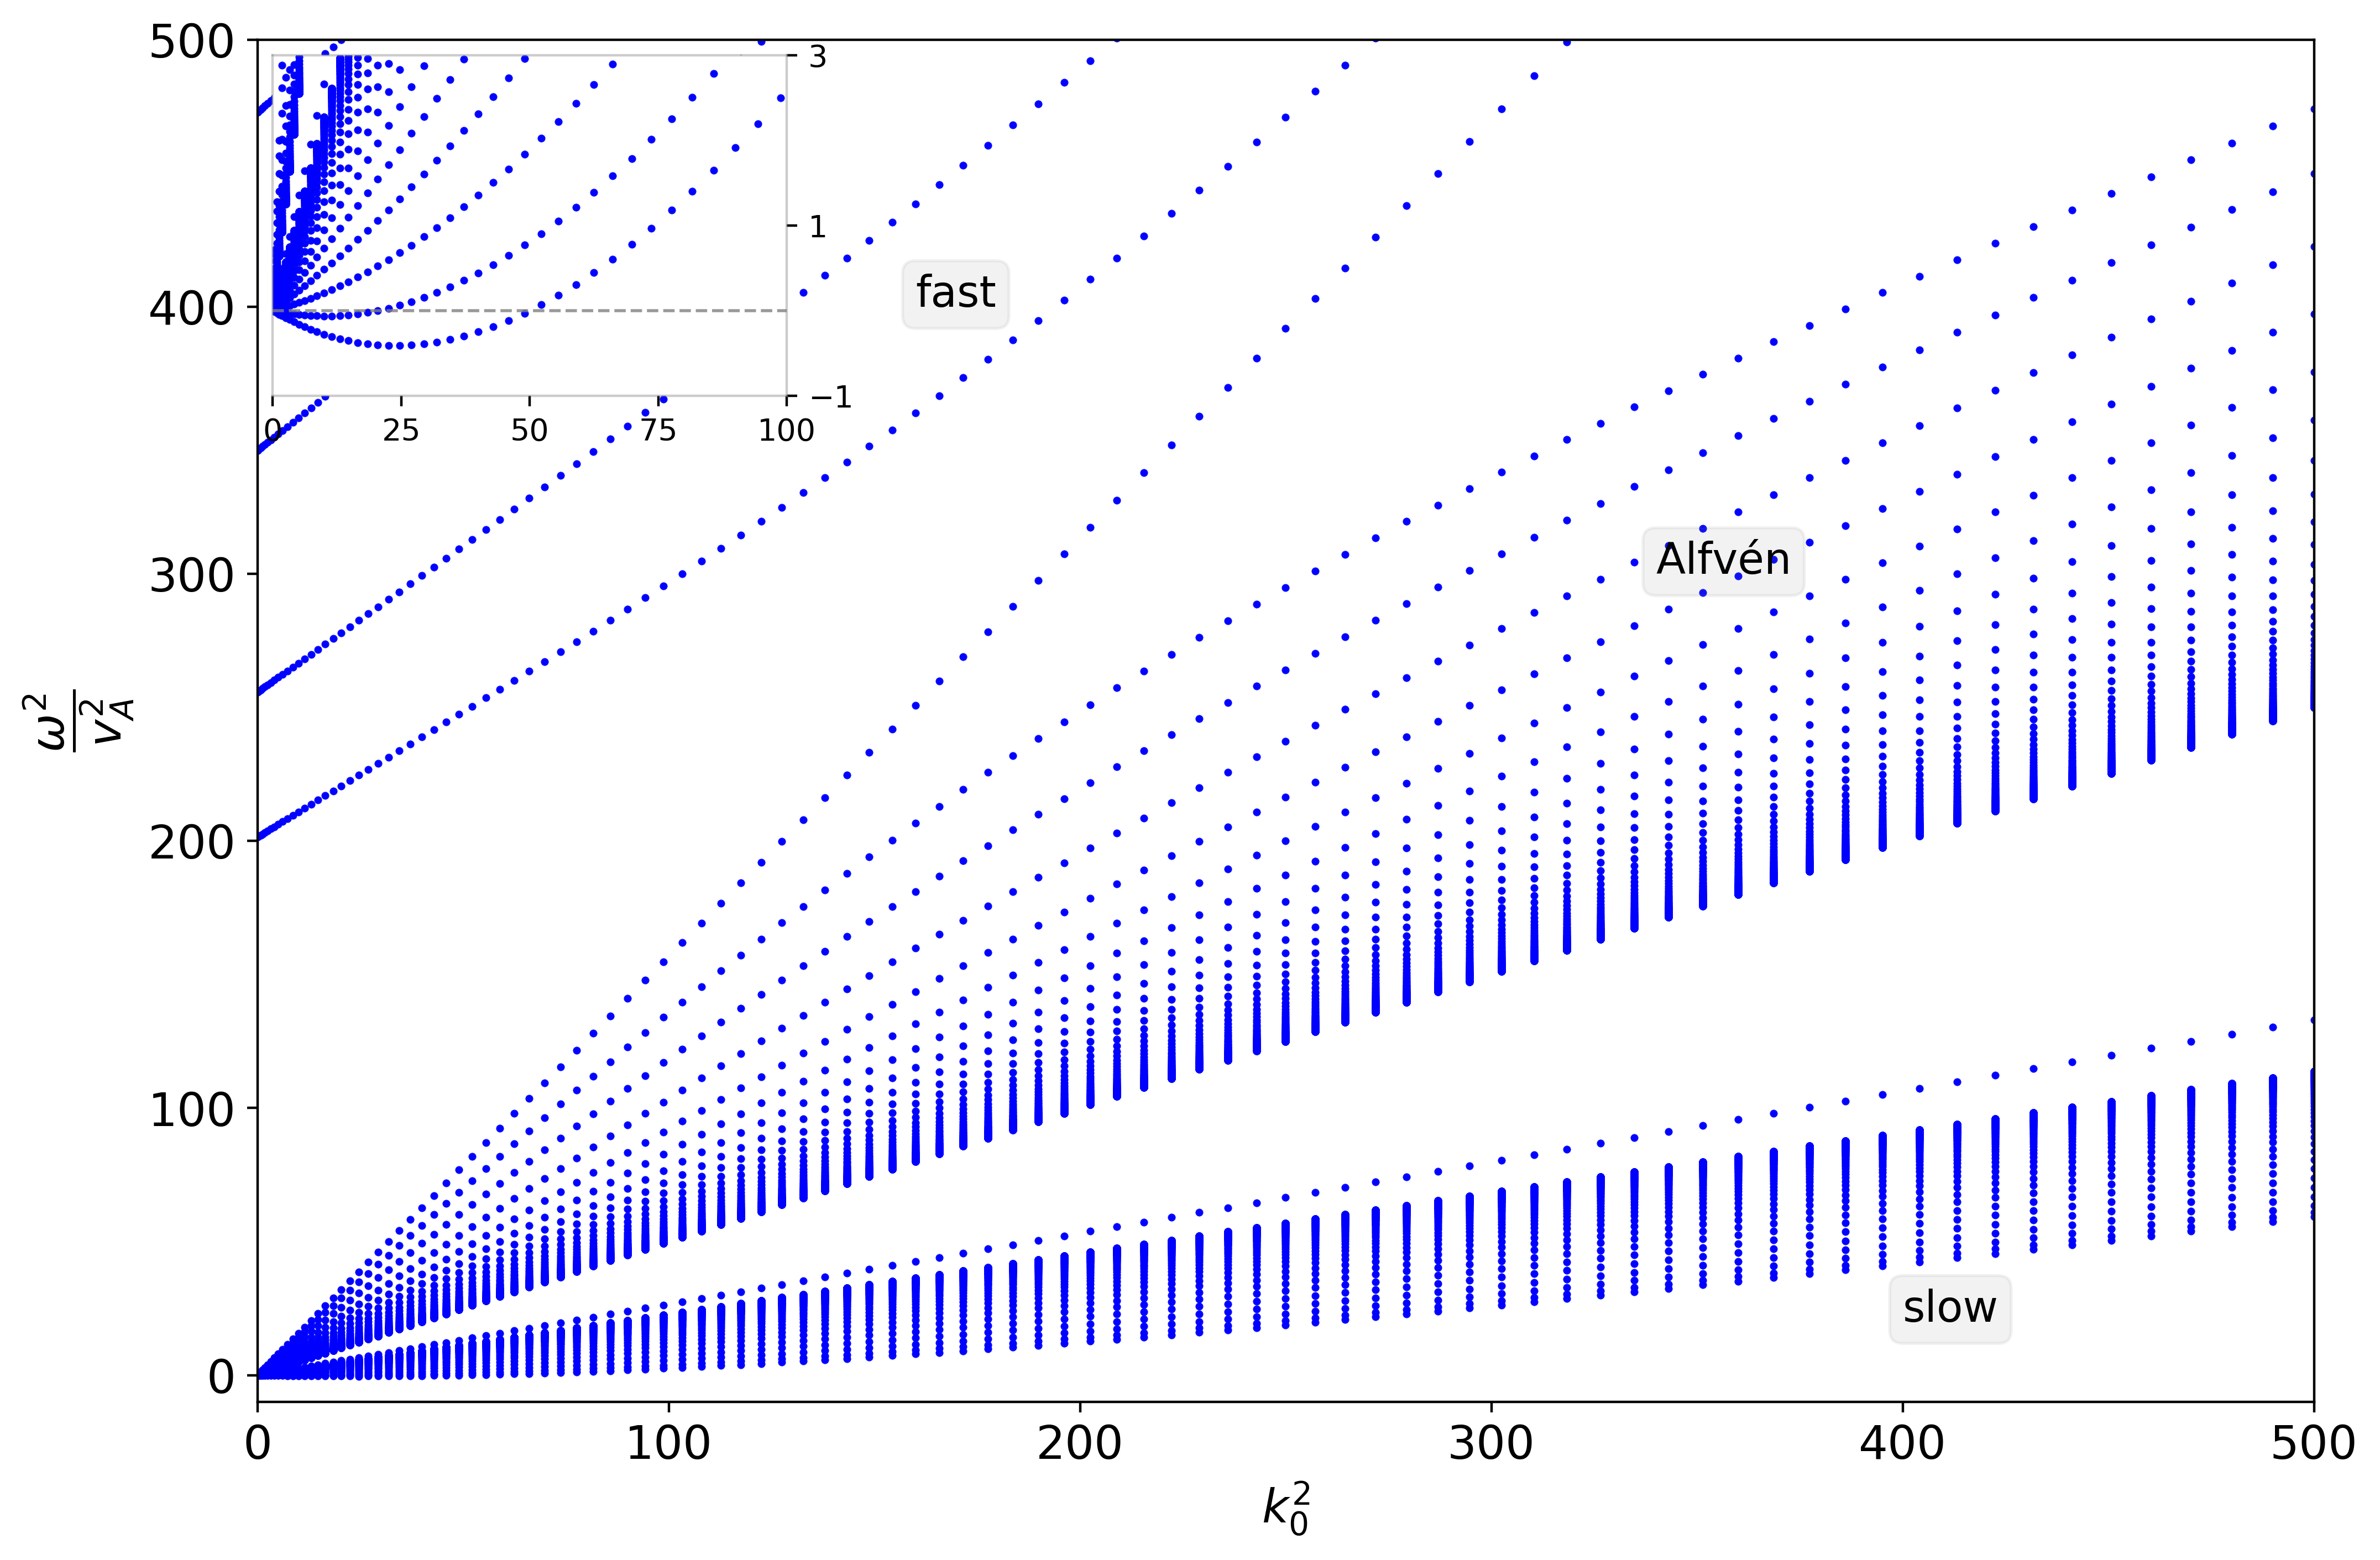
\includegraphics[width=\textwidth]{gravito_mhd.png}
  \caption{
    Spectrum of gravito-MHD modes, obtained through 100 {\legolas} runs of 351 gridpoints each. The fast (top), Alfv\'en (middle) and slow (bottom) branches of the MHD spectrum are clearly visible. The inset shows unstable slow modes at low frequencies.
  }
  \label{fig: gravito_mhd}
\end{figure}

The results are shown in Figure \ref{fig: gravito_mhd}, where every vertical collection of points at the same $k_0^2$ value represents one single {\legolas} run. Because we are in an MHD regime with a plasma $\beta = 1$, the three MHD subspectra can be clearly distinguished, showing the fast $p$ modes (top-left branches), Alfv\'en $g$ modes (middle branches), and slow $g$ modes (bottom branches). The inset shows a zoom-in near the marginal frequency of the spectrum, showing unstable $(\omega^2 < 0)$ slow MHD modes. These long-wavelength unstable modes are related to the Parker instabilities, due to magnetic buoyancy, as we will show in Section \ref{ss: quasi-parker}. Note that because this case is adiabatic and fully self-adjoint, every individual MHD spectrum is left-right and up-down symmetric in the complex eigenfrequency plane, but this aspect is hidden from the $\omega^2$ -- $k_0^2$ view shown here.


\subsection{Quasi-Parker instabilities} \label{ss: quasi-parker}
Next we discuss a modified case of the gravito-MHD waves, namely a spectrum showing quasi-Parker instabilities as done in \citet[Figure 12.2]{book_MHD}. The difference with the previous case is that a fully analytic description is no longer possible, because the introduction of magnetic shear leads to continuous ranges in the MHD spectrum. Instead of showing the spectrum for one single value for $\theta$, we now vary the direction of the wave vector $\bk_0$ between 0 and $\pi$. The equilibrium configuration is similar to the one in Section \ref{ss: gravito-mhd}, given in Cartesian geometry by
\begin{equation} \label{eq: quasi-parker}
  \begin{gathered}
    \rho_0 = \rho_c \exp\left(-\alpha x\right),
    \qquad
    p_0 = p_c \exp\left(-\alpha x\right),
    \qquad
    \alpha = \frac{\rho_c g}{p_c + \frac{1}{2}B_c}, \\
    B_{02} = B_c \exp\left(-\frac{1}{2}\right)\sin\left(\lambda x\right),
    \qquad
    B_{03} = B_c \exp\left(-\frac{1}{2}\right)\cos\left(\lambda x\right),
  \end{gathered}
\end{equation}
where magnetic shear was introduced through the parameter $\lambda$. The quantities $\alpha$ and $B_c$ are assigned the same values as in Equation \eqref{eq: gravito_mhd}; though now $g = 0.5$ and $p_c = 0.25$, which yield a plasma beta $\beta = 0.5$. The wave vectors are given by $k_y = \pi\sin(\theta)$ and $k_z = \pi\cos(\theta)$, such that $k_0^2 \approx 10$. The angle $\theta$ was varied between 0 and $\pi$ for a total of 100 runs at 351 grid points each, shown in Figure \ref{fig: quasi_parker}.

The left panels handle the case without magnetic shear, that is, $\lambda = 0$, which basically reduces to the one from the previous subsection. In this case, the slow and Alfv\'en continua collapse into single point values, denoted in red and cyan, respectively. The right panels show the same configuration where $\lambda = 0.3$ was taken, introducing magnetic shear, which introduces genuine continua seen as bands. These continua affect the overall stability and organise the entire MHD spectrum: all discrete modes are fully aware of the essential spectrum formed by these (slow and Alfv\'en) continua and the (fast) accumulation points at infinite frequency. All features of the original figure in \citet{book_MHD} are reproduced. The inset zooms into the region where both continua overlap, showing quasi-interchange and interchange instabilities. Once more, each run, shown here collectively in Figure \ref{fig: quasi_parker}, actually has a spectrum that is left-right and up-down symmetric in the eigenfrequency plane. This is depicted on Panels c and d, which show the eigenfrequency view for one single case $(\theta = 0.3\pi)$. The continuum ranges separate nicely: the collapsed single point values are denoted by cyan (Alfv\'en) and red (slow) points on Panel c, and the genuine continua are shown with cyan and red bands on Panel d. The instabilities themselves are situated on the (positive) imaginary axis, due to the self-adjointness of the eigenvalue problem.

\begin{figure}[t]
  \centering
  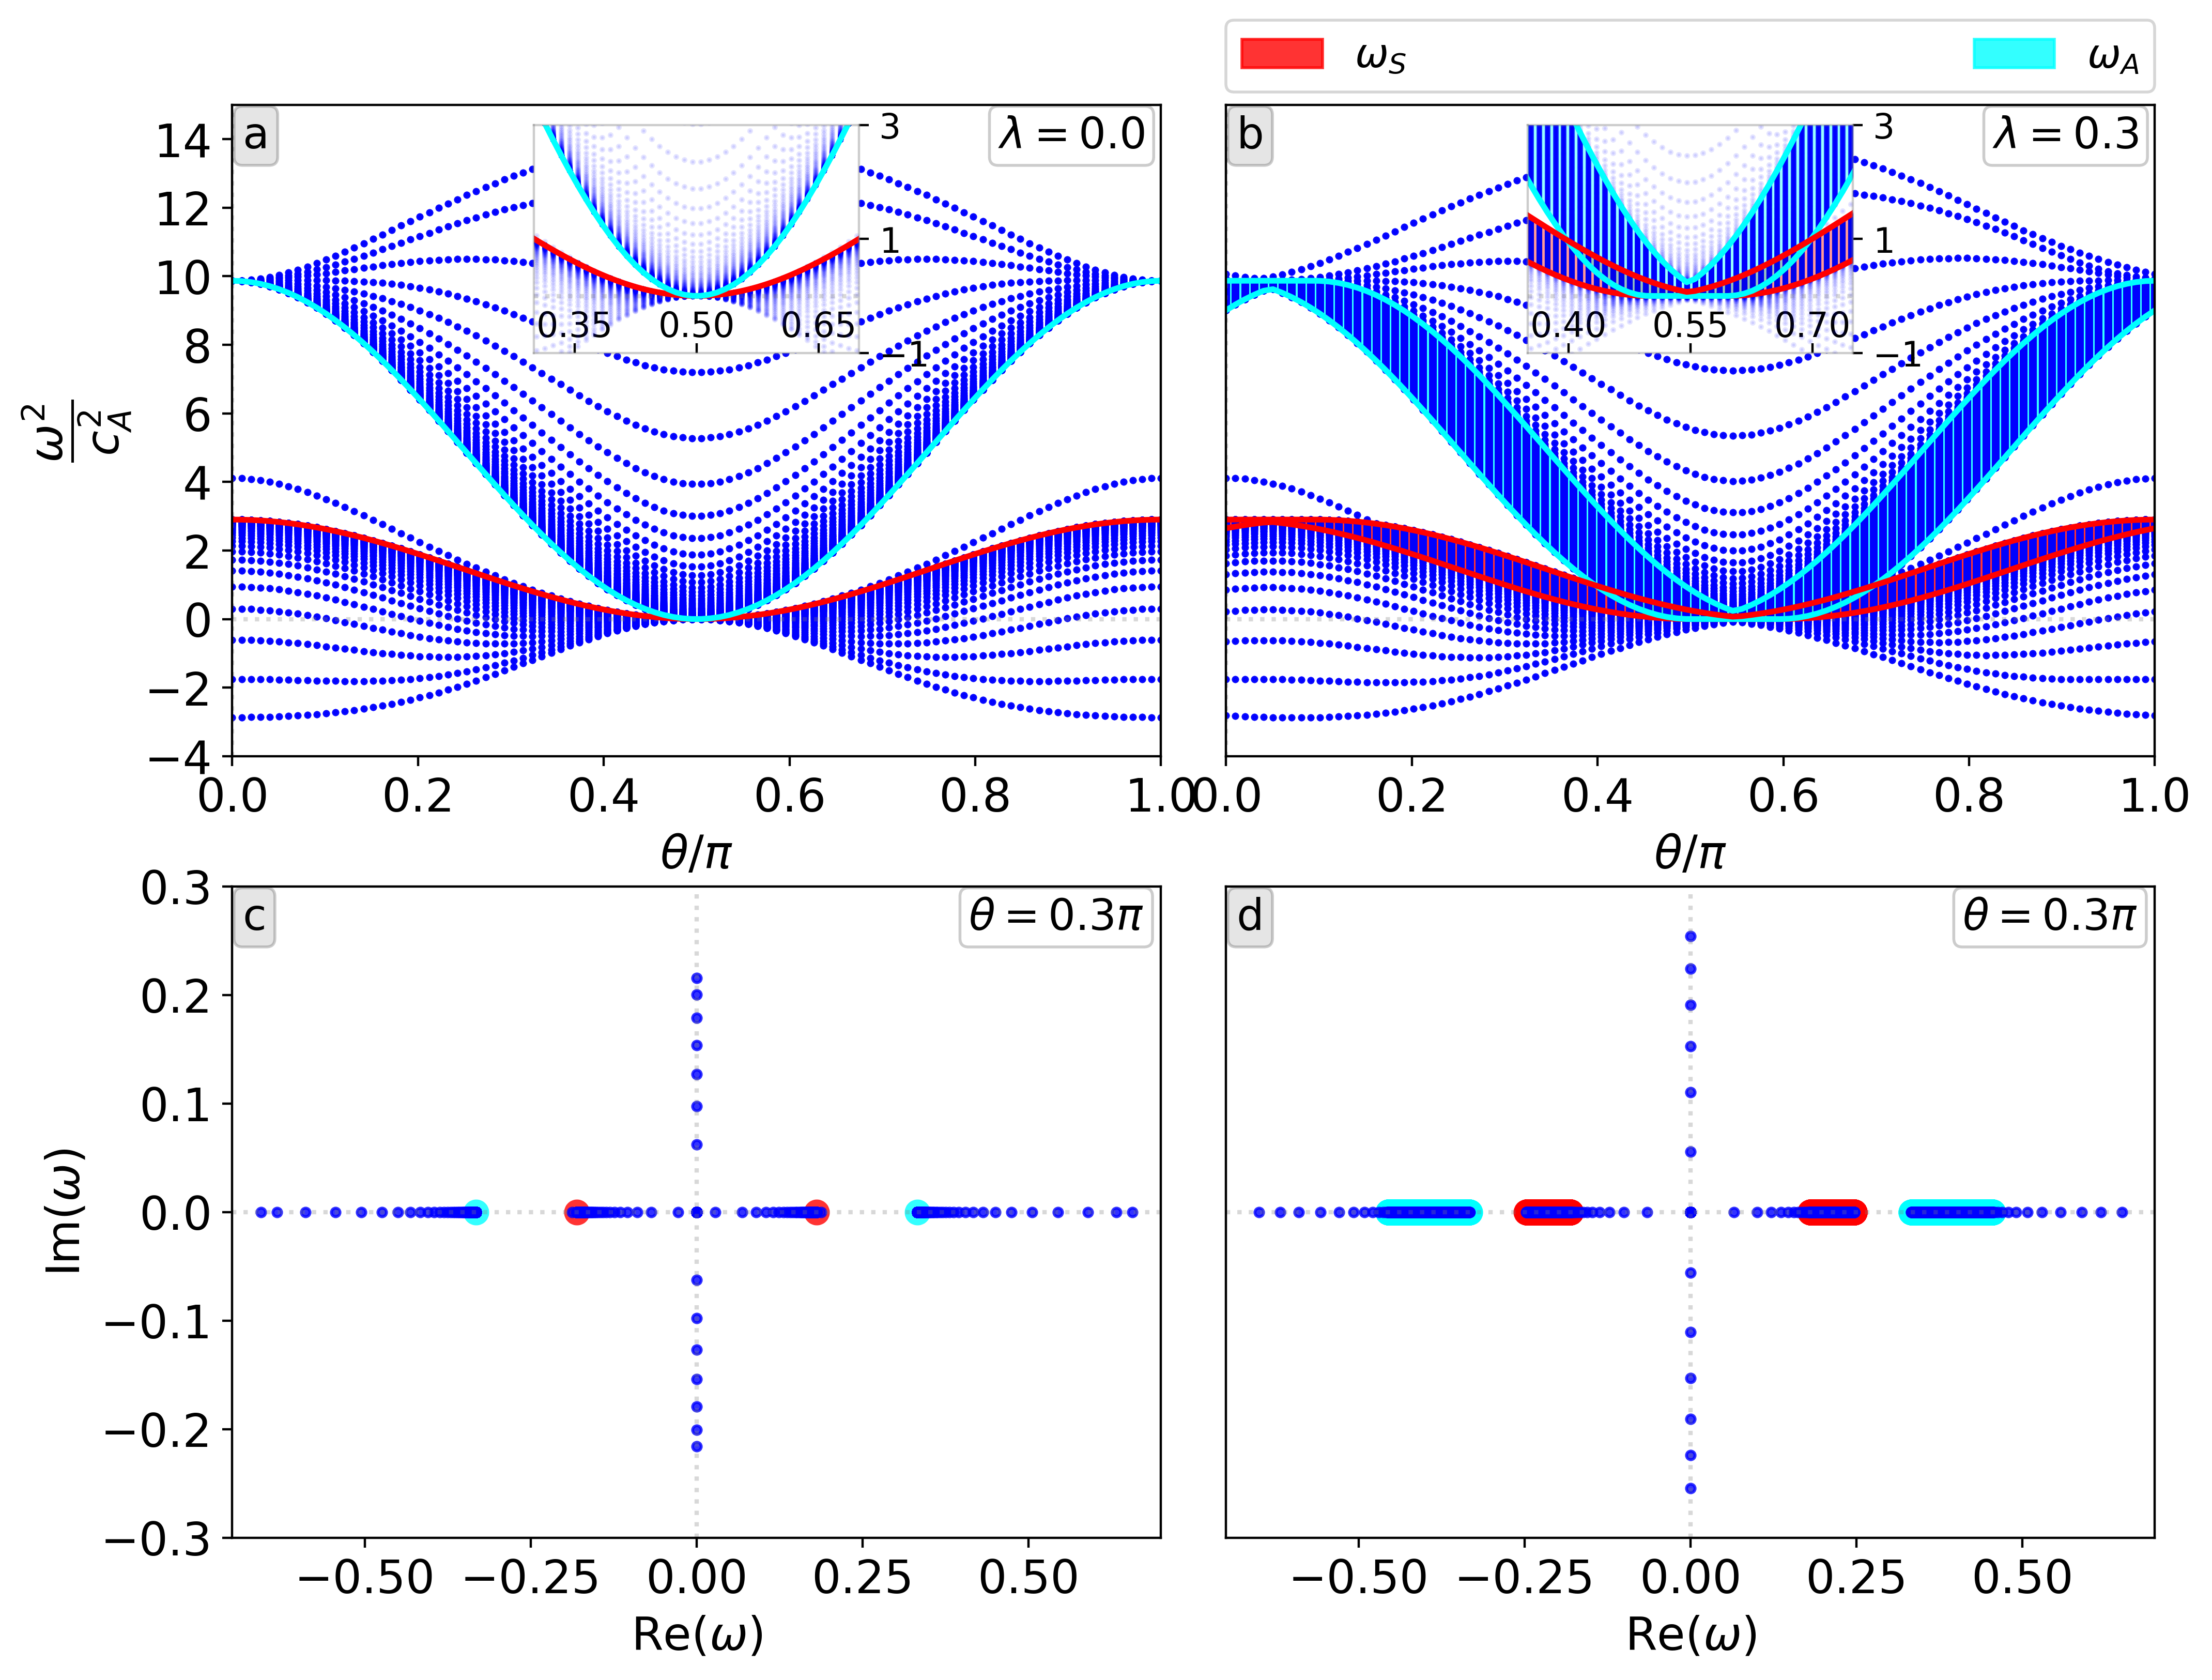
\includegraphics[width=\textwidth]{quasi_parker.png}
  \caption{
    Spectrum showing Parker and quasi-Parker modes without (\textbf{a}, \textbf{c}) and with (\textbf{b}, \textbf{d}) magnetic shear. The slow and Alfv\'en continua are shown in red and cyan, respectively, where the insets zoom into the region of quasi-interchange modes. The bottom row of panels show the eigenfrequency view for the single case $\theta = 0.3\pi$. The continua are again annotated in the panels, visualising the collapsed single point values (Panel \textbf{c}) as well as the genuine continuum ranges (Panel \textbf{d}).
  }
  \label{fig: quasi_parker}
\end{figure}

As explained in \citet{book_MHD}, we see from this eigenmode computation that the Parker instability, which is there for $\bk_0$ parallel to $\bb_0$, becomes a quasi-Parker instability away from perfect alignment and connects smoothly to well-known quasi-interchange instabilities that occur here (marginally) away from perpendicular orientation. Quantifying how the equilibrium parameters influence the growth rates of these unstable branches can only be done numerically, for example with {\legolas}.

\section{Adiabatic, cylindrical cases}
Next we move on to cylindrical configurations, which provide tests for the scale factor $\eps$ in the equations. Analytical results from the literature are again well reproduced. Furthermore, we look at different spectra previously obtained by the LEDA code, discussed in various papers, and compare those with the new spectra from {\legolas}.

\subsection{Magnetic flux tubes}
\subsection{Tokamak current profile}
\subsection{KH and CD instabilities}
\subsection{Suydam cluster modes}

\section{Resistive, Cartesian cases}
\subsection{Resistive homogeneous plasmas}
\subsection{Quasi-modes in resistive MHD}
\subsection{Resistive tearing modes}
\subsection{Tearing modes with varying resistivity}

\section{Nonadiabatic, cylindrical cases}
\subsection{Nonadiabatic discrete Alfv\'en waves}
\subsection{Magnetothermal instabilities}

\section{Convergence}

\section{The Legolas testing framework}

\section{Discussion}





\cleardoublepage
